\indent

Establishing production quality electron beam for experiments of Run Group D in Hall B is a two step process. 

\section{Beam to tagger  dump}
\indent

The initial tune is done at low currents, $<10$ nA. If the beam energy is below 6.12 GeV it is dumped on the tagger dump located under the hall's floor. If the beam energy is above 6.12 GeV  it is dumped on the "tagger-yoke dump", a dump in the tagger dipole magnet yoke, before hall proper. Beam is deflected down to this intermediate dump by the tagger dipole magnet \cite{tagger}. The tagger dipole power supply set current relates to the beam energy as \cite{yokedump}:
\begin{eqnarray}
I(A)~=~43.491\times E(GeV)-0.076
\end{eqnarray}


In this first step:
\begin{itemize}
\item the CLAS12 detectors (especially tracking detectors) must be OFF,BMT HV must be set to a SAFE mode, SVT LV should stay ON (HV OFF)
\item all halo counters must be ON
\item masked the halo counters (upstream, midstream, BOM and downstream) in beam Fast Shut Down (FSD) system 
\item the "blank" collimator with no hole is on the beam
\item the CLAS12 solenoid and torus magnets are energized (or can be be energized while beam tune is in progress)
\end{itemize}

The beam with required profile and trajectory is established by MCC OPS using correctors and quadrupoles on 2C line, while monitored by Hall-B shift crew using the wire harps and the nanoamp (nA) BPMs \cite{nA_BPM} at 2C21 and 2C24 girders in the upstream tunnel (see  Figure \ref{fig:belements}). There is a Yag viewer, ITV2C24, upstream of the tagger dipole, controlled by MCC, that may be used by MCC to verify position and profile of the beam. If the beam is tuned to the tagger dump the beam spot can be seen on the tagger dump viewer (see Figure~\ref{fig:tagger_spot}). 
Hall-B shift personnel should work with MCC operator to establish required quality beam. All harp scans must be properly analyzed and logged into logbook. The beam tune is good when required parameters for the profile (x/y widths) and trajectory (x/y positions on various monitors) are achieved. These parameters will be written on the run wiki and/or on the white board in the counting house. Typically widths at 2C21 harp $\sigma_{x,y}\le 200~\mu$m, while at 2C24 (tagger) harp $\sigma_{x,y}\le 500-600~\mu$m. In general it is a good practice to check newly measured beam parameters against last good/acceptable tune.  

\begin{figure}[htb!]
\centering
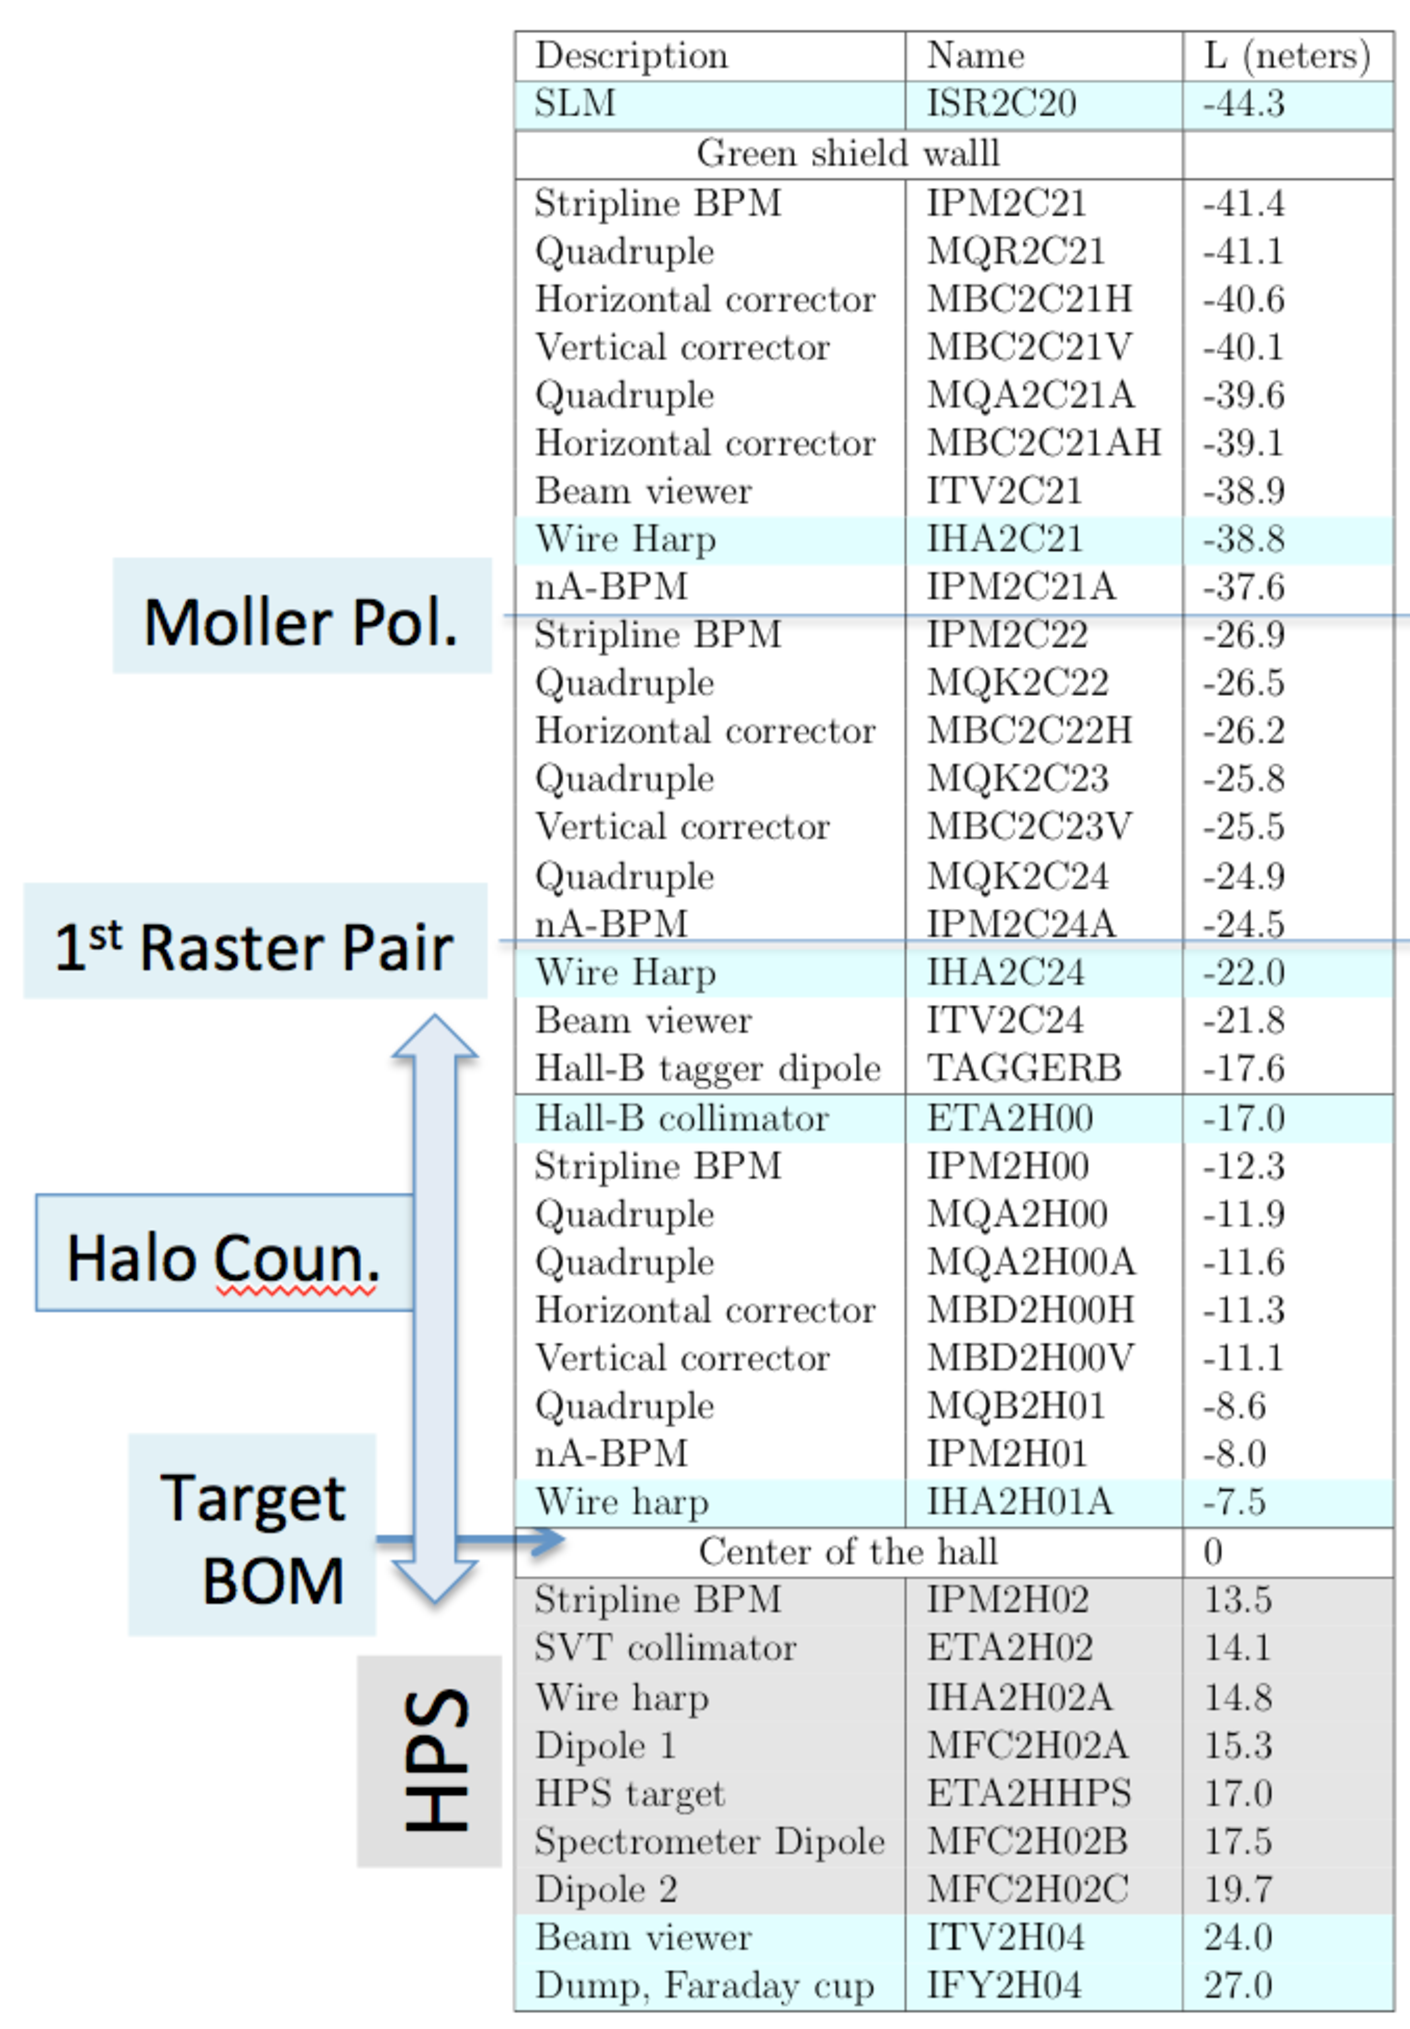
\includegraphics[width=0.8\textwidth]{beamline_elements.pdf}
\caption{Bemaline elements from the green shield wall to Faraday cup dump.}
\label{fig:belements}
\end{figure}
\begin{figure}[htb!]
\centering
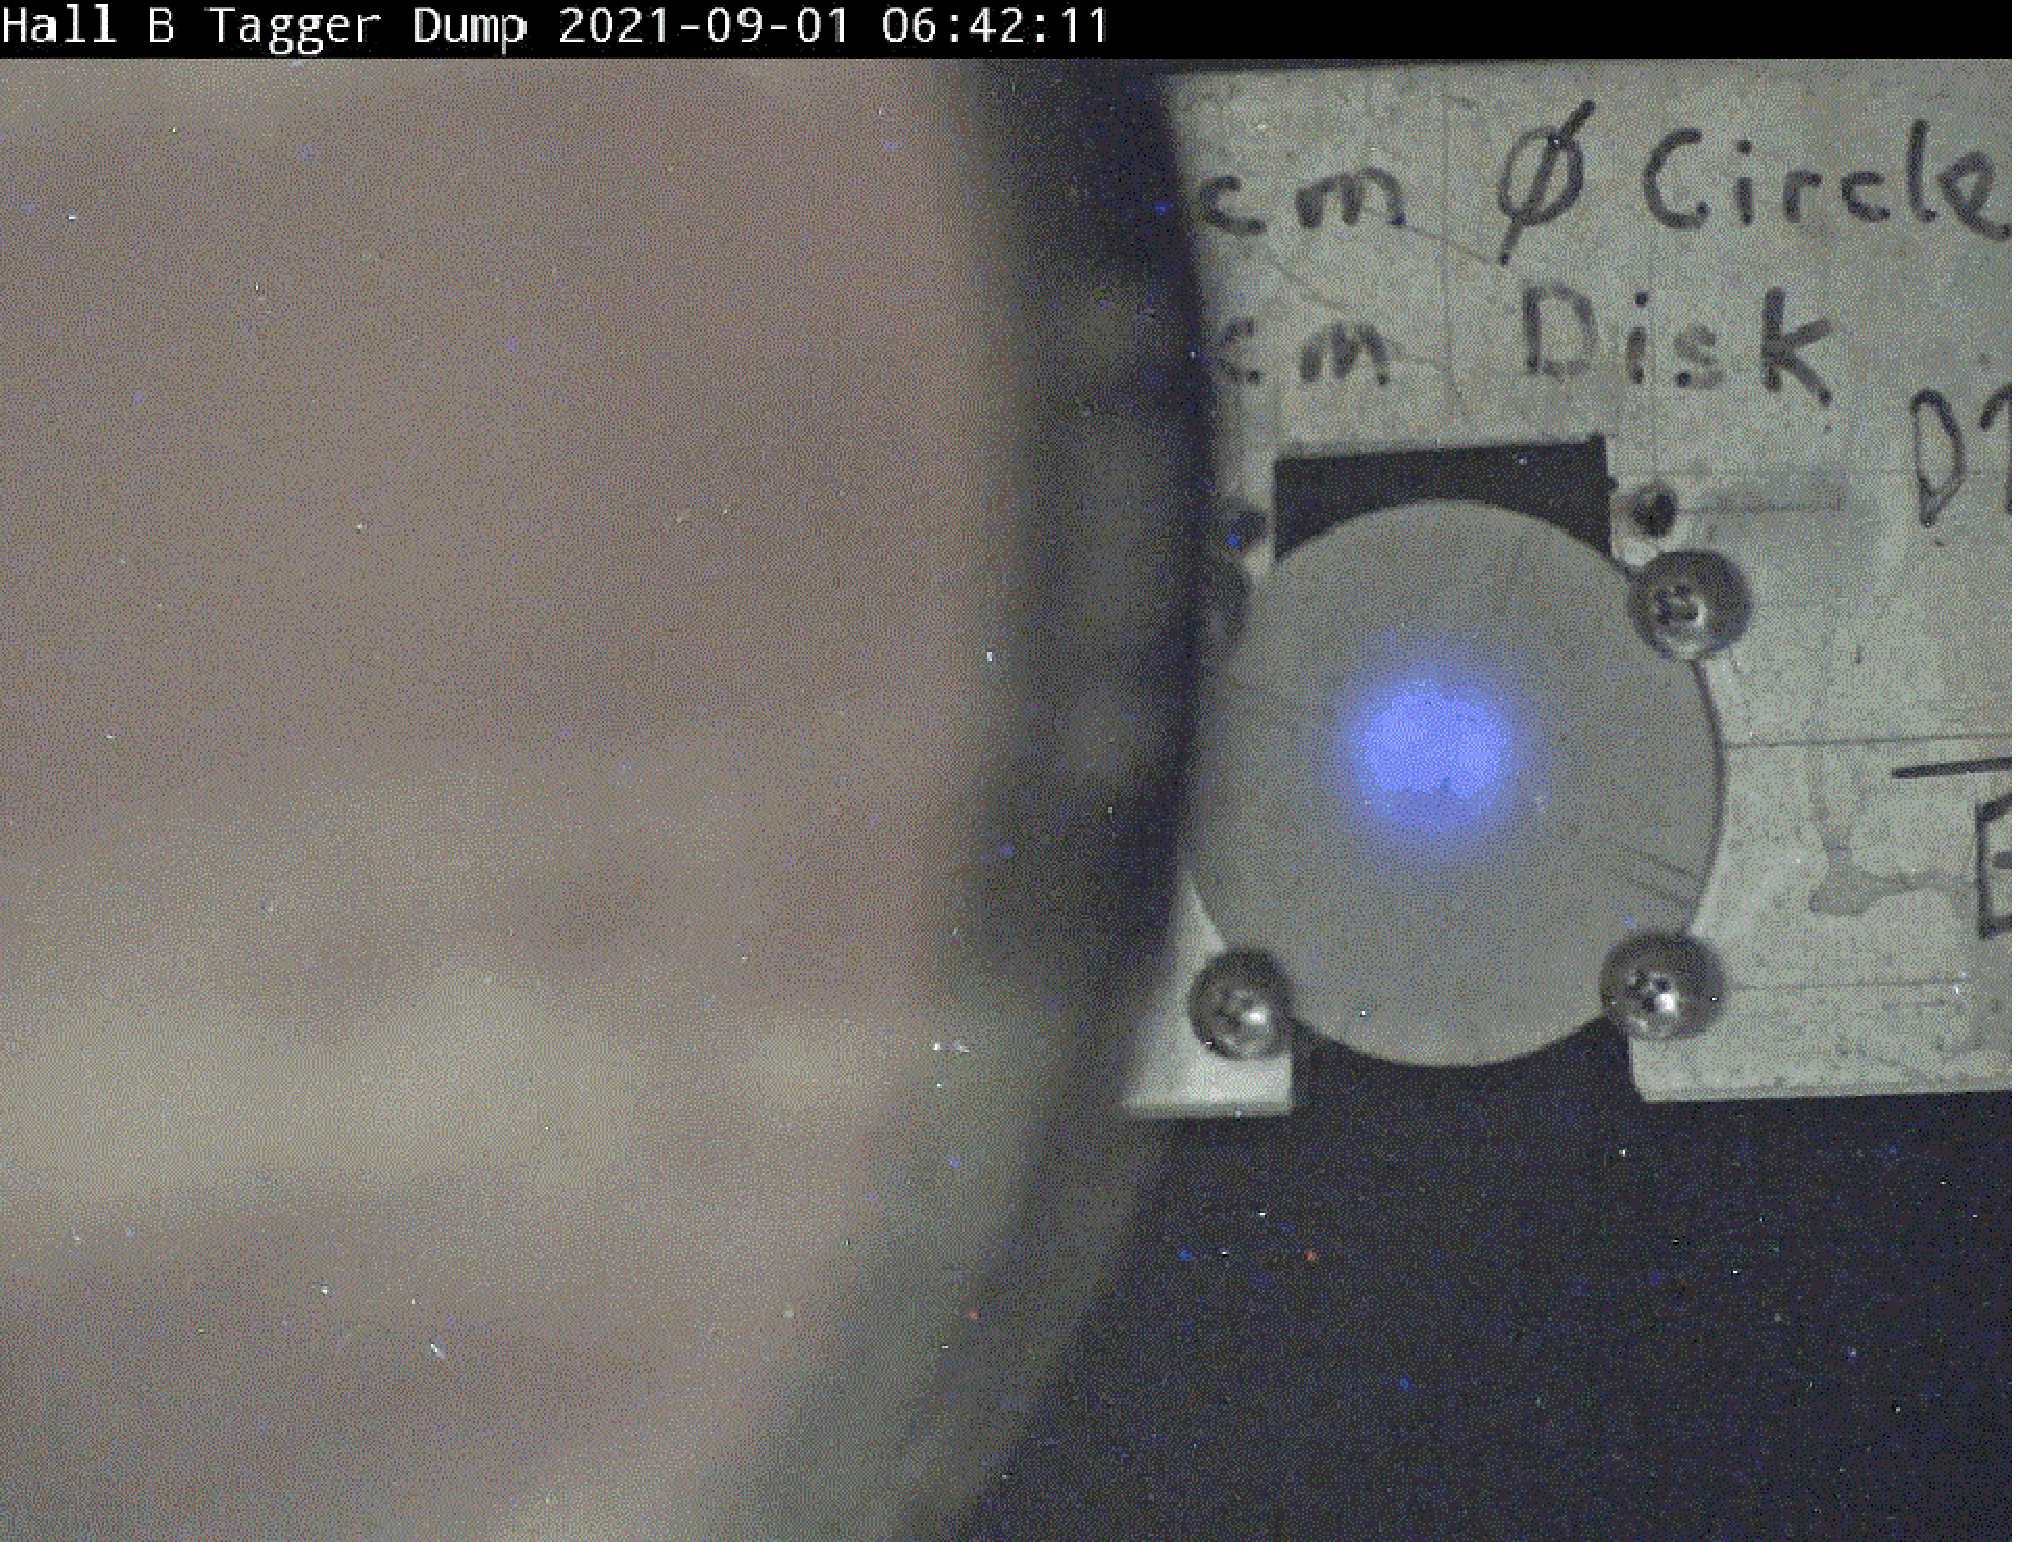
\includegraphics[width=0.8\textwidth]{Tagger_viewer.pdf}
\caption{Beam spot on the tagger dump viwer.}
\label{fig:tagger_spot}
\end{figure}


\clearpage
\section{Beam to Faraday cup}
\indent

The second step of establishing a physics quality beam starts after acceptable beam parameters have been achieved on the tagger (tagger-yoke) dump. While the tagger magnet is degaussing empty the cryotarget. If movable solid targets are used then move them out of the beam. 
The following are steps for sending beam to CLAS12:
\begin{itemize}
\item tell MCC that beam is acceptable at the tagger
\item ask to take the beam away, and degauss and turn OFF the tagger magnet 
\item position $20$ mm diameter collimator on the beam 
\item t ake the beam blocker out
\item set the halo counter FSD thresholds in to 1 MHz and the integration time interval to $50$ milliseconds
\item when ready ask MCC to send $\sim 5$ nA beam straight to the electron dump, at the end of the Hall B beamline where Faraday cup is located 
\item verify that beam goes to the dump 
\begin{description}
\item[a.] make sure beam is clearly visible on the downstream viewer, use Chromox screen\footnote{At low energies beam spot may not be clearly visible at 5 nA}. Beam should be within $10$ mm (2-tick marks) around the center (see Figure~\ref{fig:FC_spot})
\item[b.] make sure that Faraday cup beam current reading and the beam currents on 2C21 and 2C24 BPMs are consistent (the difference  should not be more then few \%)
\end{description}
\item once it is verified that the beam cleanly goes to the Faraday Cup insert the beam blocker 
\end{itemize}
\begin{figure}[htb!]
\centering
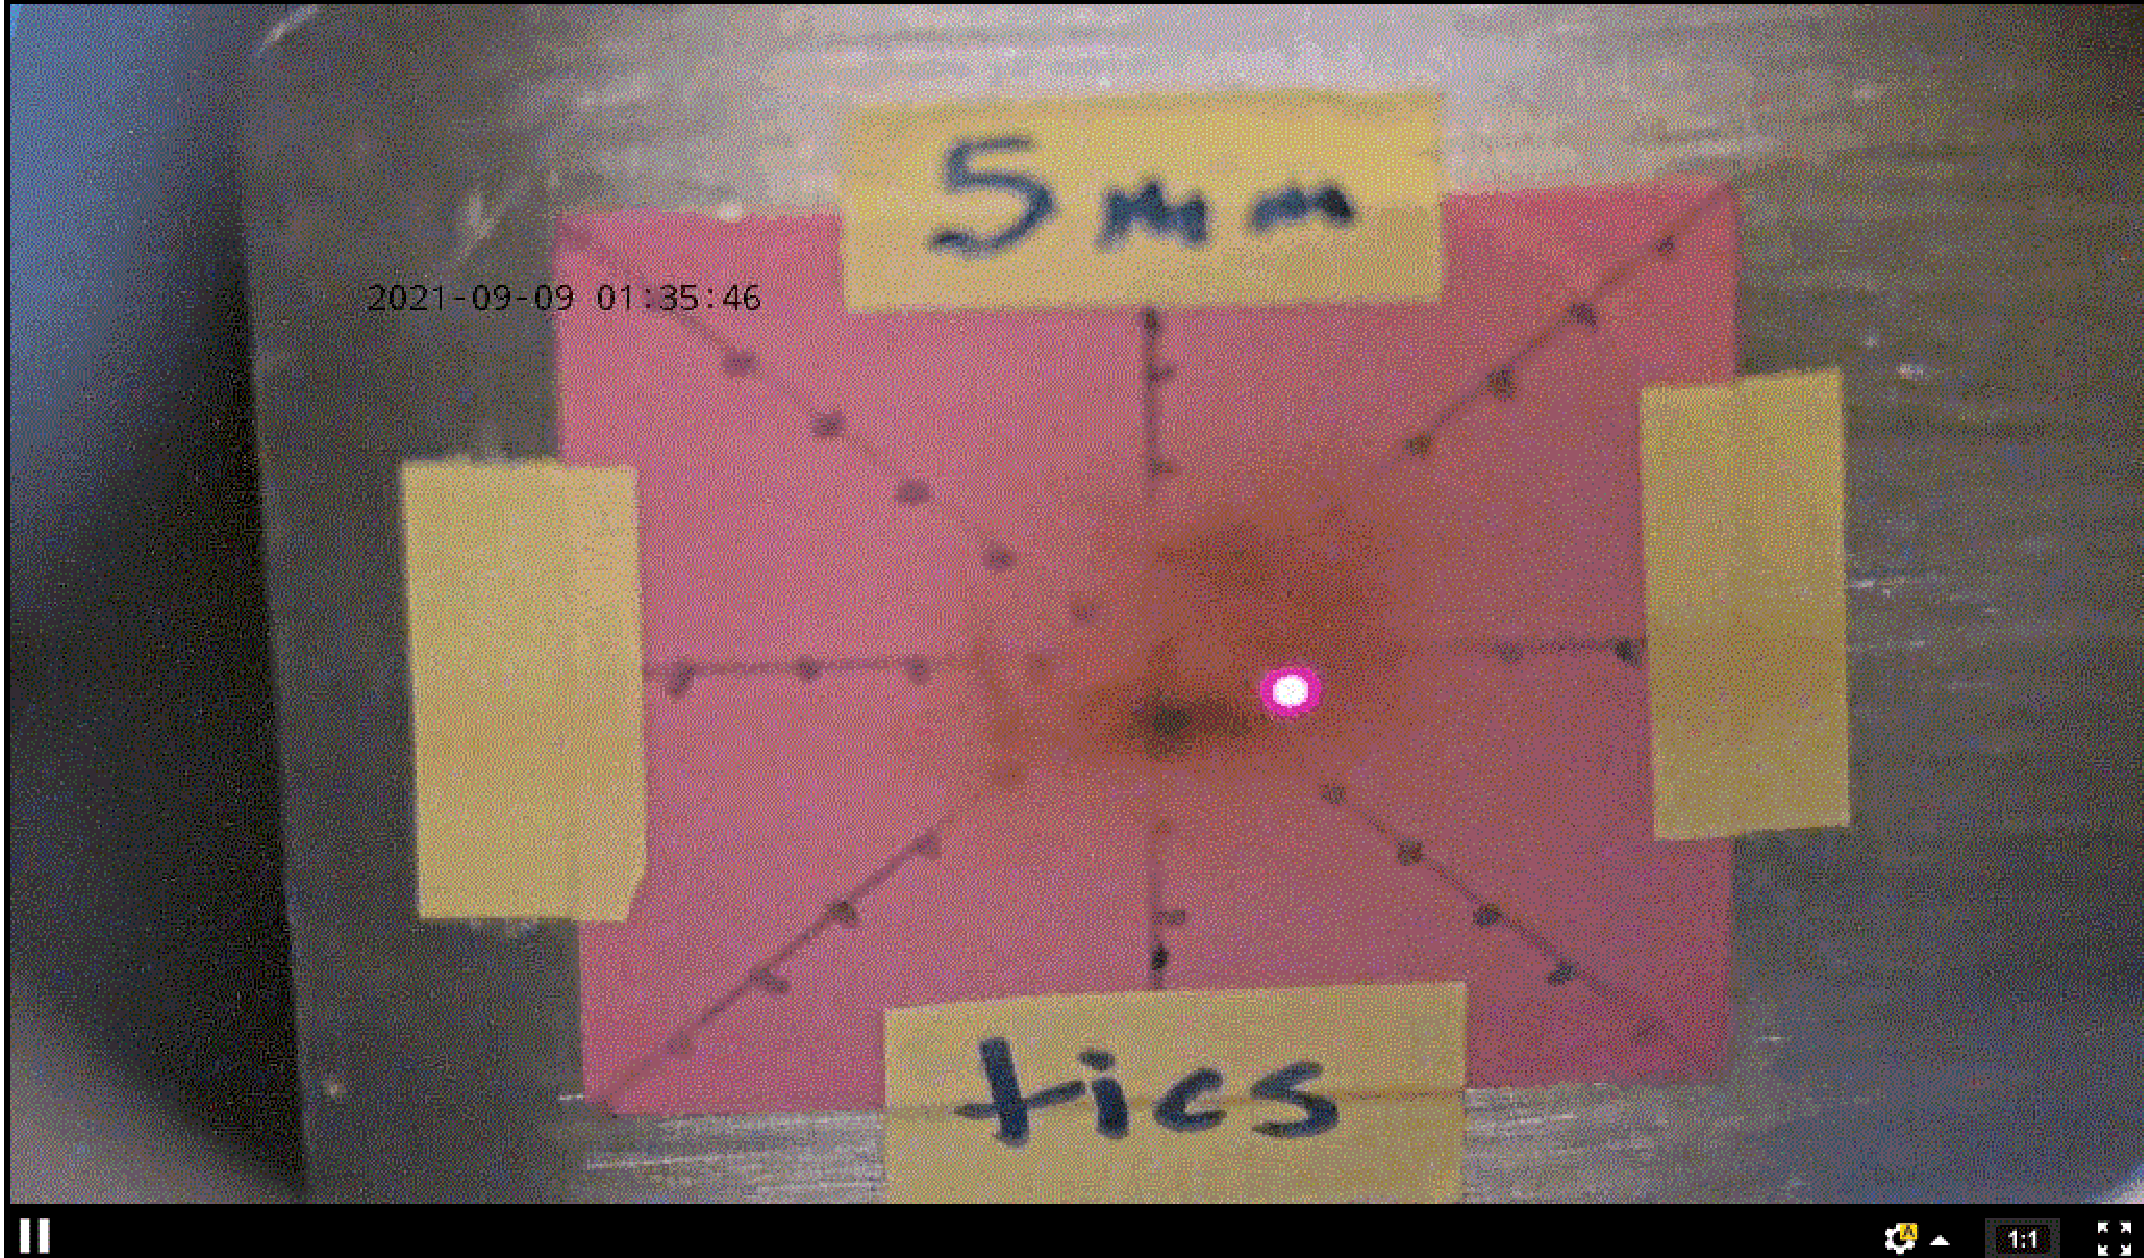
\includegraphics[width=0.8\textwidth]{FC_viewer.pdf}
\caption{Beam spot on the Faraday cup viewer.}
\label{fig:FC_spot}
\end{figure}

The beam profile and position adjustments on the target will be done using correctors and quadrupoles on 2C22/2C23/2C24 girders in the upstream tunnel and 2H00 girder in the hall (if needed). The last one is the closest to the target ($\sim 10$m upstream) and will be used to focus beam at the target location to achieve required size (preferably $<200~\mu$m). The profile and position of the beam on the CLAS12 target will be checked using a 3-wire harp 2H01A mounted about $\sim 7$ meters upstream of the CLAS12 target and 2H01 nA BPM (stripline BPM on 2H00 will not work at low currents). The 2H01A harp measures the beam profile and its projected position along x-, y-, and $45^\circ$ axes. After physics quality beam is established based on the profile, beam position on either the cryo target cell or any of CLAS12 detector component (e.g. FTcal) must be adjusted based on the lowest rates on the downstream halo counters and on BOM or symmetry of rates in the detector. 

\subsection{Procedure for adjusting the beam on the cryo target}
Run group D uses combination of liquid cell and slid foils. Schematic view is shown in Fig. \ref{fig:RGDT}

\begin{figure}[htb!]
\centering
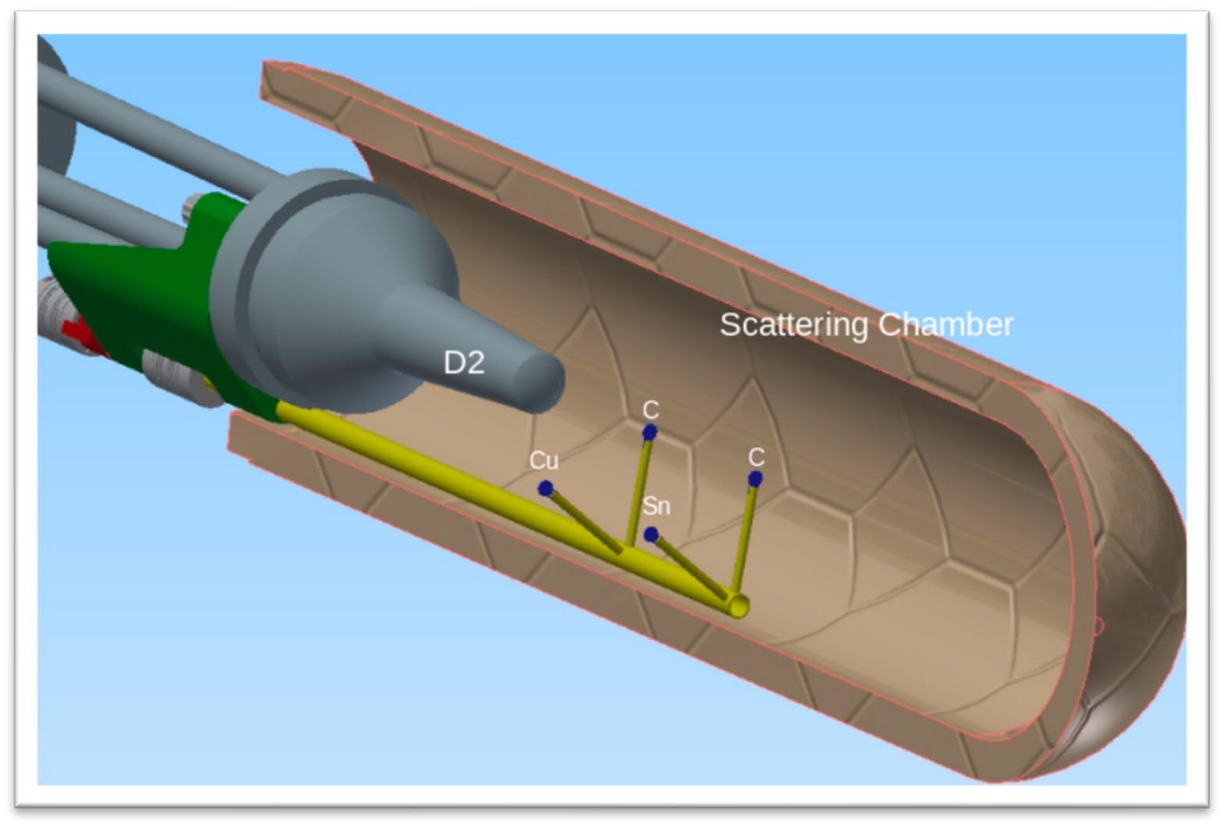
\includegraphics[width=0.8\textwidth]{RGDtarget.png}
\caption{Schematic view of the target.}
\label{fig:RGDT}
\end{figure}

Procedure for adjusting the beam on the cryo target is the following:
\begin{itemize}
\item ask MCC operator to move beam on 2H01 BPM by 0.1-0.2 mm steps up and down, vertical direction
\item record rates on halo counters and on BOM for each step. Stop moving in the given direction when rates go more more than $\times 10$ from where you started 
\item analyze rates as a function of position, find a position on 2H01 corresponding to the mid point of the two extreme ends where rates were highest. Ask MCC operator to position the beam on that position on 2H01 nA BPM
\item  repeat everything for horizontal alignment, moving the beam to left and right 
\item set orbit lock using found vertical and horizontal positions on 2H01 
\end{itemize}

The ID of the BOM is 10 mm which constrains the scan rang to less than 5 mm in any direction.

For adjusting the beam position to get symmetric rates on a detector, e.g. FTcal, move beam with small steps in x- and/or y- on 2H01 nA BPM until desired symmetry is achieved.  
\vspace{1.cm}

Once you are happy with beam position and profile document obtained beam positions on the BPMs in the logbook and proceed to the Final Steps (Section~\ref{sec:final_steps}).

\subsection{Procedure for adjusting the beam on the movable solid targets} 

The solid targets are 4 x 4 m
Target motion control GUI is shown in Figure~\ref{fig:foils}.
Procedure for adjusting the beam on the movable solid targets is the following:

\begin{itemize}
\item With solid targets out (empty position on target control GUI) of the beam request MCC to set initial beam positions on 2H01 previously obtained with cryo target. Make sure it goes cleanly to the Faraday Cup viewer and appears at the same location as with cryo target.
\item Insert solid target
\item ask MCC operator to move beam on 2H01 BPM by 0.1-0.2 mm steps left and right in horizontal direction
\item record rates on downstream halo counters for each step. Stop moving in the given direction when rates drop down more more than $\times 10$ from where you started 
\item analyze rates as a function of position, find a position on 2H01 corresponding to the mid point of the two extreme ends where rates drop. Ask MCC operator to position the beam on that position on 2H01 nA BPM
\item  similarly align beam vertically, moving the beam up until the rate drops. This is the top edge of the target
\item From this position move beam down by 1.5 mm
%\item continue moving beam down until rate increases.
\item set orbit lock using found vertical and horizontal positions on 2H01 
\end{itemize}

\begin{figure}[htb!]
\centering
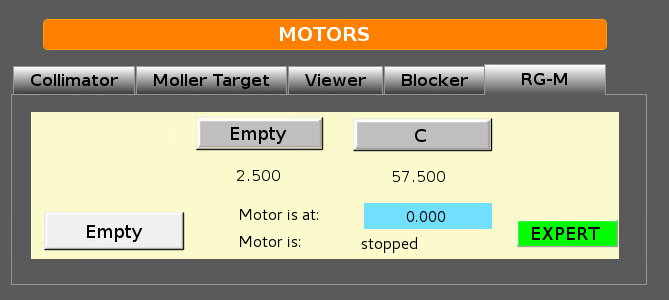
\includegraphics[width=0.4\textwidth]{1foil.PNG}
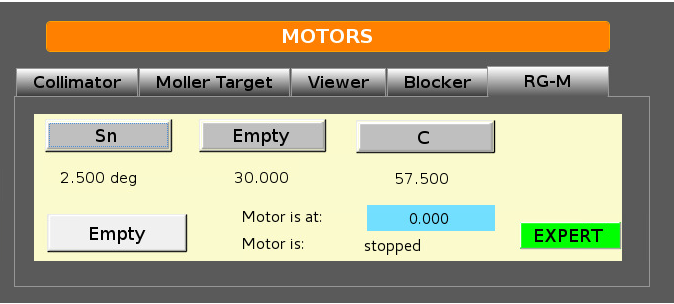
\includegraphics[width=0.4\textwidth]{2foil.PNG}
\caption{Solid target controls}
\label{fig:foils}
\end{figure}

Once you are happy with beam and target position and profile document obtained beam positions on the BPMs in the logbook and proceed to the Final Steps (Section~\ref{sec:final_steps}).



\subsection{Final steps}\label{sec:final_steps}
After high quality beam was established and properly aligned, the beam orbit lock system should be engaged. This system incorporates position readings from the BPMs (2H01 and 2H00 if currents are high enough) to regulate 
currents in the horizontal and vertical corrector dipoles to minimize beam motion at the target.  The final step in establishing the production running conditions is setting 
limits on the halo counter and BOM rates for FSD system. If beam moves unexpectedly and gets close to an obstacle, e.g. 
collimator walls or to the thick parts of the target cell, count rates on the beam halo monitors and on the BOM will increase. The appropriate rate limits will depend on actual run conditions and the target, and will be noted on the white board in the counting room and/or on the run wiki. General prescription for setting a limit for FSD input rate of N(Hz) for a trip time interval of $\delta t$ is:
\begin{eqnarray*}
N_{thr}=N+n_\sigma\times\sqrt{N\over{\delta t}}
\end{eqnarray*}
where $n_\sigma$ is how far from mean value we want the trip to acquire. For example, for $\delta t=5$ ms - the recommended value, $n_\sigma=5.$ will mean one false tripe every $5$ hour. In order to avoid frequent false trips and allow some overhead in average rate and possible smaller time interval, a recommended value is $n_\sigma=6$. Note, when beam is cleanly transported to Faraday cup, "Upstream" and "Midstream" halo counters should count $<10$ - $15$ Hz, for those FSD threshold should be set to $1000$. High rates ($\sim 100$ Hz) on these counters will indicate bed beam transport or a bleed-through from other halls and must be corrected.

